\lhead{\emph{Overview of Magnetic Field Systems}}
\chapter{Overview of Magnetic Field Systems}\label{ch:magnetics}

% \begin{itemize}
%     \item Literature Review
%     \item Literature Review of nEDM Experiments
%     \item Literature Review of Current Approaches to Magnetic Field
%     \item Magnetic Environment at TRIUMF
%     \item Magnetic Requirements for TRIUMF
%     \item Design Concepts for TRIUMF
% \end{itemize}


In Chapter~\ref{ch:motivation}, the motivation behind nEDM experiment alongwith measurement principle of nEDM have been described. The TUCAN nEDM experiment has been also introduced there. This chapter describes about the magnetic requirement for the TUCAN nEDM experiment. It also describe the magnetic subsystems which are required to maintain the label of precision for the experiment to be successful. Moreover, the chapter also described the current nEDM status worldwide and also the use of active shielding for nEDM measurement. Finally, the chapter ends with  describing the main objective for this thesis. 

 \section{Magnetic field requirements for the TUCAN nEDM experiment}\label{sec:msr}
% To achieve $10^{-27}$ e$\cdot$cm sensitivity level for TUCAN nEDM experiment, it must be ensured to have a magnetic field of $\sim$1 pT stability i.e. $<$pT drift in one nEDM measurement cycle and $\sim$1 nT/m homogeneity. So, the magnetic field should be precisely monitored and controlled which imply that the coil generating the field must be better than that level. The nEDM experiment itself along with passive shielding will be under a Magnetically Shielded Room (MSR) and around which compensation coils will be placed for active shielding which needs to be designed as shown in Fig. \ref{fig:msr}. 
% A stable and homogeneous magnetic field $\bm{B_o}$ ($\sim$1 $\mu$T) is required to achieve the desired $10^{-27}$ e$\cdot$cm sensitivity level for TUCAN nEDM experiment. 

A stable and homogeneous magnetic field is required for the TUCAN nEDM experiment. The magnetic field should be precisely monitored and controlled which imply that the coil generating the field must be better than that level. The magnetic stability upper limit is $\sim$1 pT i.e. $<$pT drift in one nEDM measurement cycle and the magnetic homogeneity upper limit is $\sim$1 nT/m. For compensating $\bm{B_0}$ field fluctuations,  $^{199}Hg$ co-magnetometer will be used. To nullify the uncontrolled and time-varying external fields both active and passive shielding will be utilized. The nEDM experiment itself along with passive shielding will be under a Magnetically Shielded Room (MSR) and around which compensation coils will be placed for active shielding which needs to be designed. The schematic diagram of the magnetic components of the
TUCAN nEDM experiment is shown in Fig.~\ref{fig:msr}. Each of the magnetic component is explained below. 


\fig{Images/msr_pic}{width = \textwidth}{Schematic diagram for the TUCAN nEDM magnetics. From inside out: The UCN and the co-magnetometers followed by the internal coil system (  $\bm{B_0}$ and B $\bm{B_1}$ coils) to generate the magnetic fields for the Ramsey cycle. Outside to that there are four layers of passive shielding which made the magnetically shielded room (msr). The active compensation system which needs to be designed is just outside the msr.\label{fig:msr}}
 
% As explained in Section~\ref{sec:lim} and Section~\ref{sec:nEDM} that to achieve $10^{-27}$ e$\cdot$cm sensitivity level for TUCAN nEDM experiment, it must be ensured to have a magnetic field of $\sim$1 pT stability and $\sim$1 nT/m homogeneity. So, the magnetic field should be precisely monitored and controlled which imply that the coil generating the field must be better than that level. The nEDM experiment itself along with passive shielding will be under a Magnetically Shielded Room (MSR) and around which compensation coils will be placed for active shielding which needs to be designed as shown in Fig. \ref{fig:msr}. 
%  \fig{Images/exp2}{width = 0.8\textwidth}{Schematic diagram of prototype active compensation system at University of Winnipeg.\label{fig: active}}



% \doublefig{Images/msr_pic}{width =\textwidth,height =7cm}{Schematic diagram \label{fig:msr_pic}}{Images/msr_sketch}{width = \textwidth,height =7cm}{Photograph\label{fig:msr_sketch}}{{Schematic diagram for the TUCAN nEDM magnetics. From outside in: The
% active compensation system followed by several layers of magnetically shielded room and
% passive shields nullify the environmental magnetic eld. The magnetometers inside the
% active shielding monitor the changes in the magnetic eld internal to that region. The
% internal coil system (B0 and B1 coils) generate the magnetic elds for the Ramsey cycle.
% The UCN and the co-magnetometers are internal to the coils. } \label{fig:msr}}

\FloatBarrier


%  Furthermore, a multi-layer passive shielding system must reduce and stabilize the field around the internal coil. Self-shielded $\bm{B_0}$ coils and shim coils are the options for internal coils around the nEDM cells due to their immunization capability from the field perturbations that is induced by the changes in the magnetic permeability of the passive shields arising from temperature fluctuations \cite{Andalib_temp}. The passive shielding's magnetization must be tailored with degaussing and the shields themselves stabilized mechanically and thermally.  Finally, the magnetic environment of the passive shielding system must be stabilized.  The active shielding will control the magnetic field immediately outside the outermost passive shielding layer.   This thesis came into play for possible designing concepts of active shielding which will be discussed next.


% to the $\pm$ 1 nT level in the 10 Hz to DC frequency range. 


\subsection{Co-magnetometer}
Comagnetometry enables a measurement of the magnetic field inside the nEDM cell while the nEDM measurement is being conducted. It is the only way to correct for possible false EDM's caused by time-varying leakage currents. 

A comagnetometer is used to measure and correct for  $\bm{B_o}$ field drifts. The comagnetometer is an atomic species (usually $^{199}\text{Hg}$). In the comagnetometer, optical pumping is used to polarize a vapor of mercury atoms  which are then intoduced into the
nEDM cell at the same time as the neutrons, and the spin-precession frequencies of both species are measured simultaneously. Comagnetometer and neutrons motion in the EDM cell in the presence of a magnetic gradient causes frequency shifts that reverse sign with $\bm{E}$ reversal \cite{comag_1,comag_2,comag_3}. Both the comagnetometer and UCN are affected, but comagnetometer effects tend to dominate due to the higher (thermal) velocity of the atoms. So, precession frequencies of the comagnetometer can be used to normalize the magnetic field drifts. Normally, drifts of 1-10 pT in $\bm{B_o}$ field may be corrected using the comagnetometer technique in a typical nEDM experiment. The design of the $^{199}\mathrm{Hg}$ comagnetometer in the TUCAN ndem experiment will be similar to that employed in the previous ILL nEDM experiment \cite{bestLim_1,comag_4}.


Besides that a number of atomic magnetometers are placed just outside the
nEDM measurement cell. They are used to characterize magnetic homogeneity and stability. The chief purpose is to characterize gradients, in order to characterize the leading contributions to false EDM's arising from Hg and UCN motion in the EDM cell.

\subsection{Internal Coils}

A static $\bm{B_0}$ field ($\sim$1 $\mu$T) as well as an oscillating $\bm{B_1}$ field ($\sim$30 Hz) are required in the Ramsey Resonance method for $\pi$/2 spin reorientation. In addition, shim coils which carry a relatively small current are required to null remnant transverse fields and gradients over the nEDM measurement cell

$\bm{B_0}$ coils will be based on self-shielded coils which prevent eddy currents (loops of electrical current induced by a changing magnetic field) from being generated in the first place. The self-shielded $\bm{B_0}$ coils and shim are considered to be installed in the msr due to their immunization capability from the field perturbations that is induced by the changes in the magnetic permeability of the passive shields arising from temperature fluctuations \cite{Andalib_temp}. High-precision current supplies ($\sim$ 1 ppm) will be used to drive all internal coils, regardless of design. AC coils will apply $\pi$/2 pulses for the UCN and comagnetometer species, to initiate free spin precession.



\subsection{Passive Shield}\label{sec:passive}
The task of the passive magnetic shielding system is to provide a magnetically stable environment to perform the precision low field NMR spectroscopy on the neutrons. The TUCAN nEDM experiment will employ a magnetically shielded room (MSR) consisting of four nested mu-metal enclosures as its passive shielding, conceptually similar to Ref.~\cite{msr_design}.  The passive shield is designed so that the magnetic fields inside are stable enough to be be measured by
our precision comagnetometer and magnetometers discussed earlier. 

% It includes a degaussing/idealization system used to reduce remnant magnetization in the shield layers which further improves the stability.

During quiet times at TRIUMF, fuctuations in the magnetic feld are $\sim$100 nT. An MSR with a quasi-static shielding factor of $\sim$ 100,000 is sufficient to reduce these fuctuations to the $\sim$ pT level, beyond which a comagnetometer must be used to correct the field to the $\sim$ 10 fT level. A four-layer MSR with an inner cubic space of side-length 1.8 m and outer side-length 2.8 m produces this shielding factor, with mu-metal wall thicknesses 2 mm, 6 mm, 4 mm, 4 mm (inner to outer), equally spaced.


\subsection{Active Magnetic Field Compensation (AMC)}\label{sec:amc}

The environment of the TUCAN nEDM experiment needs to be thermally and vibrationally isolated and controlled, primarily to avoid small changes and slow drifts in the properties of the passive magnetic
shielding. 

A particularly challenging aspect is that the TUCAN nEDM experiment will be in fringe field of TRIUMF cyclotron, at a location where the fringe could be as large as eight times the magnetic field of the earth ($\sim\;400\;\mu T$) with  fluctuations $\sim\;100\;nT$ due to external magnetic sources such as nearby beam line magnets or the displacement of large magnetic objects (e.g.,
the crane is the Meson Hall).

Fluctuations can be compensated using a system of magnetic sensors and coils to characterize and control the environment around the magnetic shields in a feedback loop. The TUCAN's plan is to reduce the static field to less than 50 $\mu$T using dedicated compensation coils and constant-current supplies, with a readily achievable stability of $\mathrm{10^{-3}}$ and to reduce the remaining static field and fluctuations by up to a factor of 100 through a separate set of compensation coils and current supplies, using fluxgate magnetometers
for magnetic feedback. The fluxgate sensors will be placed in the region
between the compensation coils and the passive shields. The PSI~\cite{bea}
and Munich~\cite{lins} groups have both commissioned and characterized such systems. The PSI group has also presented designs of their planned system for the n2EDM upgrade~\cite{rawlik}.

The active shielding will control the magnetic field immediately outside the outermost passive shielding layer. Overall, the active shielding system should be able to reduce the net background magnetic field to the level of tens of nT over the volume of the nEDM cell. This thesis came into play for possible designing concepts of active shielding which will be discussed in the following Chapters.



% At large fields, saturation of the passive magnetic shielding system can be a concern, which would seriously impact its effectiveness. Furthermore, when accessing the experiment, the door to the MSR must be opened. If presented with a large external field, the innermost layer of the passive shielding system could themselves become magnetized, necessitating degaussing and additional experimental down time with these factors in mind. The proposed plan is to nullify and stabilize the magnetic field environment at TRIUMF to ($\sim\;1\;\mu T$) using dedicated large bucking coils and also to reduce the fluctuations upto a factor of 100 using a separate set of coils by supplying currents to them  where the fluctuations will be measured by fluxgate sensors in a continuous feedback loop. Moreover,
% every channel  going through the feedback loop must be sampled faster than goal correction rate which is 6 Hz. The goal correction rate is set by :

% \begin{itemize}
%     \item  Precision frequency of the species in the experiment which is Hg-199 larmor frequency at 1 $\mu$ T.
%     \item  Induction of correction coils sets fundamental settling time.
%     \item  Correction for changes due to the sources in Meson Hall of TRIUMF where the actual experiment will take place .
%     \item  Change of earth's field with time.
% \end{itemize}

\section{Experimental Efforts So Far}\label{sec:lim}
\fig{Images/lim}{width = \textwidth}{Experimental nEDM upperlimit over the years \cite{1_lim,2_lim,3_lim,4_lim,5_lim,6_lim,7_lim,8_lim,9_lim,10_lim,11_lim,12_lim,13_lim,14_lim,15_lim,16_lim,17_lim} along with theoretical predictions \cite{theory_lim_1, theory_lim_2, theory_lim_3}. The vertical dashed line indicates the introduction of UCN. The light green region indicates the the nEDM limit in SUSY, M-theory and others while he light red region indicates for SM. \label{fig:lim}}

Additional sources of CP violation beyond the standard model predict the nEDM to be in the range of $10^{-27}$ -- $10^{-28}$  e$\cdot$cm as compared to $10^{-33}$ -- $10^{-31}$ e$\cdot$cm predicted by the standard model \cite{theory_lim_1, theory_lim_2, theory_lim_3}. There are several experiments aiming at improving the uncertainty on the nEDM. The Fig. \ref{fig:lim} summarize all the results. Since the first measurement data published in 1957 \cite{1_lim}, the upper limit set on nEDM has been reduced by eight orders of magnitude over the last six decades. At 1980, ultra cold neutron (UCN) experiment overtook over neutron beam experiments on precision. The current best upper limit set by ILL/Sussex/RAL nEDM experiment is $3.0 \times 10^{-26}$ e-cm (90 \% C.L) or $3.6 \times 10^{-26}$ e$\cdot$cm (96 \% C.L)  \cite{bestLim_1,bestLim_2} and the experiment is performed at Institut Laue-Langevin (ILL, Grenoble, France). The new $^{199}\mathrm{Hg}$ EDM measurement constrains the nEDM better than direct nEDM measurements, $d_n$ $<$   $\mathrm{1.6\times10^{-26}}$ e$\cdot$cm, although subject to uncertainty from
Schiff screening~\cite{schiff_screen}. The TUCAN nEDM experiment is aiming to constrain the uncertainty on the nEDM at the $10^{-27}$ e$\cdot$cm sensitivity level. 

The Paul Scherrer Institut
(PSI, Villigen, Switzerland) nEDM experiment uses an improved version of the former 
ILL/Sussex/RAL single-cell apparatus. Several innovations have been made at PSI, including a new SD2 spallation-driven UCN source. The experiment employs several Cs magnetometers outside the EDM cell, and a $^{199}\mathrm{Hg}$ comagnetometer. Active magnetic shielding and other environmental controls have been improved. A new detector that can simultaneously count both spin states of UCN has also been implemented. The final sensitivity expected
is $\mathrm{10^{-26}}$ e$\cdot$cm~\cite{psi}. Some of the chief improvements made at PSI recently have been in the area of nearby alkali atom (Cs) magnetometry, Hg comagnetometry, and neutron magnetometry. A recent achievement at PSI is the understanding of the Cs magnetometer signals in terms of magnetic field gradients internal to the magnetic shielding. This has led to a detailed understanding of the false EDM of the Hg comagnetometer~\cite{psi_falseEDM}. Another recent achievement is in using the neutrons themselves to measure gradients~\cite{psi_n_gradient}. PSI also aims to improve their magnetometry with $^3\mathrm{He}$ magnetometers inside the electrodes of the double EDM measurement cells for their future n2EDM effort. They have performed R$\&$D using Cs magnetometers to sense the free-induction decay signal from $^3\mathrm{He}$, which resulted in a new high-precision magnetometer possessing excellent long-term stability\cite{psi_magnetometer}. The precision goal for n2EDM is $5 \times 10^{-28}$ e$\cdot$cm~\cite{psi_n2edm_nEDM-workshop,psi_n2edm_PPNS-workshop}.



The nEDM collaboration at Spallation
Neutron Source (SNS, Oak Ridge, TN, USA) plans to measure $d_n\approx$ $2\times10^{-28}$ e$\cdot$cm, two orders
of magnitude improvement from the current limit~\cite{sns_lim}. They plan to use a unique experimental technique. A Cold Neutron (CN) beam from the SNS will impinge upon a volume of superfluid $^4\mathrm{He}$ creating UCN. The nEDM measurement will also be conducted in the superfluid. A small amount of polarized $^3\mathrm{He}$ introduced into the superfluid $^4\mathrm{He}$ will
act as both a comagnetometer and spin analyzer for the UCN. The $^3\mathrm{He}$ neutron capture rate is strongly spin dependent, and will beat at the difference of the Larmor precession frequencies of the neutrons and $^3\mathrm{He}$. A non-zero EDM would change the beat frequency with E-reversal. Scintillation light produced in the superfluid will be used to detect the capture products. The target precision is $10^{-28}$ e$\cdot$cm The false EDM of the $^3\mathrm{He}$ comagnetometer may be reduced by collisions in the surrounding $^4\mathrm{He}$~\cite{sns_false_edm}. The group aims to
commission the experiment at SNS by 2020.

A new room-temperature nEDM experiment will be conducted using an upgraded
Los Alamos National Laboratory (LANL, Los Alamos, NM, USA) UCN source~\cite{lanl_nEDM-workshop}. The aim of the project is to increase the UCN density by a factor of five to ten, which could then be used to carry out a $\sim$ $10^{-27}$ e$\cdot$cm determination
of the nEDM. The experiment aims for completion of a $10^{-27}$ level result, to be completed in the years prior to the SNS nEDM experiment, which shares a number of collaborators. Two other room temperature nEDM experiments are being pursued at the Forchungsreaktor Muncheon II (FRM2) reactor in Munich~\cite{frm2} and Gatchina reactor at ILL~\cite{PNPI}. Both experiments feature double measurement cells and Cs magnetometers internal to the innermost magnetic shield. The Munich effort features an impressive new effort in active and passive magnetic shielding~\cite{msr_design,shield_pnpi,shield_pnpi2}, and uses $^{199}\mathrm{Hg}$ comagnetometer. The ILL/Gatchina experiment has produced results at ILL~\cite{PNPI}. This could be improved in further runs at ILL in the EDM position, or in runs using the superfluid He UCN source at ILL, where a statistical sensitivity of $3.5 \times 10^{-27}$ e$\cdot$cm could be obtained~\cite{pnpi_nEDM-workshop}. The group will build a UCN source at the WWR-M reactor in Gatchina in order to increase the UCN 
flux.

\section{Review of the AMC System Worldwide for nEDM Measurement}

The active magnetic magnetic compensation system has been first commissioned and characterized by the PSI group where the detail process has been written in the PhD thesis of the Ref.~\cite{bea} in 2013. The PSI's nEDM experiment is shielded from the outside magnetic field via a four-layer cylindrical shield
of Mu-metal. To reduce and stabilize the outer magnetic field to keep the magnetization of the Mu-metal in a stable state, they build a AMC system known as surrounding field compensation (SFC) system. There they use 
six 6m$\times$8m rectangular coils creating three orthogonal pairs which will act as compensation coils. The currents in these coils
can be controlled dynamically via a proportional-integral feedback loop. A regularized, pseudoinverse matrix of proportionality factors, which correlate magnetic field changes at given sensor positions to current changes in the SFC coils, is incorporated in the feedback loop. This approach is superior to simpler feedback controls, and the magnetic field can be stabilized
by roughly one order of magnitude within a large control volume and not only at single points. The system that they described is pioneer for other AMC systems doe nEDM measurement. But the system doesn't provide clear solution to the possible placements of the fluxgates. They claim that having more sensors than coils produce better compensation but they have not the clearly uses the matrix condition nymber or coil design. In 2018, the flaws of that system have been pointed out by another student of the same group in his PhD thesis~\cite{rawlik}. There, a well conditioned matrix has been discussed by new coil design. The author in Ref.~\cite{rawlik} also claims that there is no need of Proportional (P)-Integral(I) or simply PI feedback algorithm which turns out to be false.

Besides that in 2016, the Munich group has also characterized such a system where the where the detail process has been written in the PhD thesis of the Ref.~\cite{lins}. The work described their was similar to that in Ref.~\cite{bea} in terms of matrix inversion. They have also talked about the different coil designs. They had 24 coils and 180 field probes for active shield.

Moreover, before the work in this thesis came into play, another thesis from our collaboration (TUCAN) had been written by Ref.~\cite{mike} in 2013. He introduced the development of active magnetic shielding for TUCAN nEDM measurement. He talked about the PID control while there was no shield present.


% The experiment has been done at the Institut Laue-Langevin (ILL) which is situated at Grenoble, France. A new generation of UCN source known as superthermal UCN source which uses a new method of cooling by transferring energy to quantum excitations in a material have recently come online. To use such a UCN source, the nEDM appa

% The apparatus for nEDM experiment has been moved from ILL to a superthermal UCN source at Paul Scherrer Institut (PSI) which is situated at Villigen, Switzerland. UCN superthermal source use the cooling technique . A new UCN source generation have recently come online. They use a technique from condensed
% matter physics involving cooling by transferring energy to quantum excitations in a material.
% UCN sources that employ this method of cooling are known as superthermal sources and they are
% beginning to transform the landscape of fundamental neutron physics at various facilities in the
% world.
% The nEDM apparatus from ILL was moved to such a UCN source at Paul Scherrer Institut
% (PSI, Villigen, Switzerland). The apparatus was also improved and upgraded in several respects.
% Data-taking for this new nEDM experiment was completed recently and the analysis of the data is
% ongoing [9]. The expectation in the community is that this new result will improve the previous
% best by a factor of about three to four.
% Next generation UCN EDM experiments are now in preparation at a variety of sites aiming to
% improve the result by an order of magnitude or more. Experiments are either ongoing or planned
% at ILL [10, 11], PSI [12], the Gatchina reactor [10], the Forchungsreaktor Munchen II (FRM2)
% reactor [13], Los Alamos National Laboratory (LANL, Los Alamos, NM, USA) [14], the Spallation
% Neutron Source (SNS, Oak Ridge, TN, USA) [15], and our eort at TRIUMF [16, 17]. We discuss
% our relationship to these experiments in Section 4. Our goal of dn < 10��27 ecm within the next
% 6-7 years (running until 2024-25, as stated earlier) is competitive with these eorts. One of the key
% factors is our unique UCN source, which we are upgrading. We envision achieving UCN counting
% rates over 100 times larger than the previous best nEDM experiment and the recently completed
% experiment at PSI, and similar to or surpassing the plans of other experiments.





\section{Overview of The Thesis}
The goals to design an AMC system as explained in section \ref{sec:amc}  are the following:
\begin{itemize}
    \item  To stablize the magnetic field surrounding  MSR $\leq\;100\;nT$ and for that sample every channel in the feedback loop more than 6 Hz.
    \item  To reduce $\sim\;400\;\mu T$ background field to avoid saturation
    \item  To able to open the door without magnetizing internal layers.
\end{itemize}

The overall objective of this thesis is to focus on the the development and testing of AMC prototype so that the above mentioned goals can be implemented for the actual experiment at TRIUMF. The AMC prototype has been set up at University of Winnipeg and tested at a highest possible way within the last three years time frame and expalined in Chapter \ref{ch:amcP}. The main focus has been given on the stablization of the surrounding field fluctuations and understanding every problems that have been faced with possible solutions. Mainly, the work has been done by closely following the work of PhD thesis \cite{bea,lins,rawlik} as explained in Chapter \ref{ch:operation}. However, while studying those theses, some faults have been discovered which are considered as the achievements for this thesis as explained in Chapter \ref{ch:quantification}. Finally, Chapter \ref{ch:conclusion} talks about the future work that could be done and how the thesis will be milestone for future studies before summarizing everything.


% \section{Concept of Active Compensation}

% \fig{Images/exp2}{width = 0.8\textwidth}{Schematic diagram of prototype active compensation system at University of Winnipeg.\label{fig: active}}


% \newcommand{\fig}[4]{\begin{figure}[h]
% \centering
% \includegraphics[{#2}]{{#1}}
% \caption{#3}
% \end{figure}}

% \begin{figure}
%     \centering
%     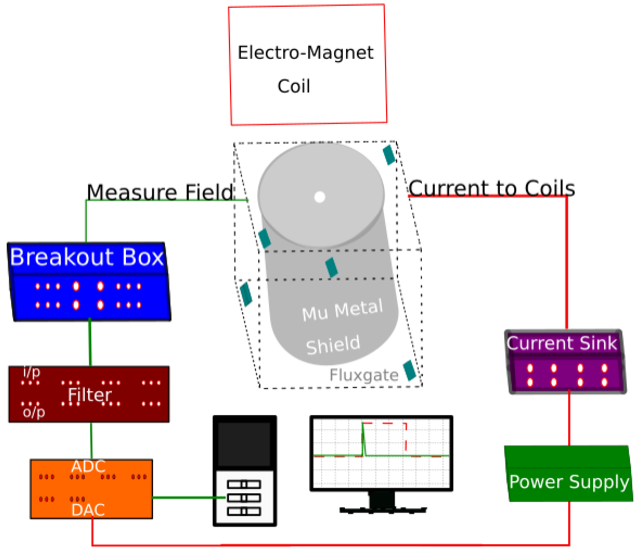
\includegraphics[width=0.4 \textwidth]{Images/exp}
%     \caption[width=0.4 \textwidth]{Schematic diagram of prototype active compensation system at University of Winnipeg . }
%     \label{fig:active shielding}
% \end{figure}
% \begin{figure}
%     \centering
%     \includegraphics[width=0.5 \textwidth]{Images/ss}
%     \caption[width=0.4 \textwidth]{PI loop in flow chart. First measurement from the fluxgates will act as set-point. Then the repeated measurements from the fluxgates are taken. For each measurement difference with the setpoint are noted. On the basis of the difference, the required amount of current for the coils surrounding the outermost layer of the shileding are determined and sent. Those coil currents generate required amount of magnteic flux to compensate for the differences.}
%     \label{fig:active shielding}
% \end{figure}
% The four layer Mu-metal cylinder enclosing the experimental area, which will be used for passive shielding has surrounded by six coils on six faces , each of having 1 mm$^2$ area. The outermost cylinder with coils surrounding it has been shown in the Fig.\ref{fig: active}. The magnetic environment is sensed by the fluxgates placed in different positions on the surface of the coils. The fluxgates that have been used are 3-axis. So, a breakout box has been built to separate each of x,y $and$ z axis in respective direction. Then, a fourth order low pass butterworh filter with cutoff frequency at 10 Hz has been built  to get rid of high frequency noise. After filtering,  the signals are transmitted to the computer via analog to digital converter (ADC) of LabJack T7 Pro for controlling via proportional integral (PI) feedback loop. 

